\documentclass[tikz, border=20pt]{standalone}

\usepackage{fontspec}
\setsansfont{Inter}[
  BoldFont=Inter Bold,
  Scale=0.92
]

\usepackage{tikz}
\usetikzlibrary{
  shapes.geometric,
  arrows.meta,
  positioning,
  fit,
  calc,
  backgrounds,
  shadows.blur
}

% --- IBM Carbon palette ---
\definecolor{primary}{HTML}{0F62FE}
\definecolor{teal}{HTML}{009D9A}
\definecolor{orange}{HTML}{FF832B}
\definecolor{purple}{HTML}{8A3FFC}
\definecolor{green}{HTML}{198038}
\definecolor{cyan}{HTML}{0072C3}
\definecolor{magenta}{HTML}{D02670}
\definecolor{surface}{HTML}{F4F4F4}
\definecolor{border}{HTML}{A8A8A8}
\definecolor{textprimary}{HTML}{161616}
\definecolor{textsecondary}{HTML}{525252}
\definecolor{arrowcolor}{HTML}{6F6F6F}

% Layers
\pgfdeclarelayer{background}
\pgfsetlayers{background,main}

% Subtitle command
\newcommand{\nsub}[1]{{\sffamily\tiny\color{textsecondary}#1}}

% --- Styles ---
\tikzset{
  base/.style={
    text=textprimary,
    font=\sffamily\small,
    align=center,
    inner sep=8pt,
  },
  service/.style={
    base,
    draw=#1!60,
    top color=#1!4,
    bottom color=#1!12,
    rounded corners=6pt,
    minimum width=3cm,
    minimum height=1.3cm,
    line width=1.2pt,
    drop shadow={
      shadow xshift=0pt,
      shadow yshift=-2pt,
      opacity=0.15,
      fill=black
    },
  },
  service/.default=primary,
  stor/.style={
    base,
    cylinder,
    shape border rotate=90,
    aspect=0.3,
    draw=#1!60,
    top color=#1!4,
    bottom color=#1!14,
    minimum width=2.4cm,
    minimum height=1.6cm,
    line width=1.2pt,
    drop shadow={
      shadow xshift=0pt,
      shadow yshift=-2pt,
      opacity=0.15,
      fill=black
    },
  },
  stor/.default=primary,
  step/.style={
    base,
    draw=#1!60,
    top color=#1!4,
    bottom color=#1!12,
    rounded corners=5pt,
    minimum width=2.6cm,
    minimum height=1.1cm,
    line width=1.2pt,
    drop shadow={
      shadow xshift=0pt,
      shadow yshift=-1.5pt,
      opacity=0.12,
      fill=black
    },
  },
  step/.default=teal,
  container/.style={
    rounded corners=10pt,
    fill=surface,
    draw=border!50,
    line width=0.6pt,
    inner sep=14pt,
  },
  clabel/.style={
    font=\sffamily\scriptsize\bfseries,
    text=textsecondary,
    anchor=north west,
  },
  flow/.style={
    -{Stealth[length=6pt, width=5pt]},
    line width=1.4pt,
    draw=arrowcolor,
  },
  flowlight/.style={
    -{Stealth[length=5pt, width=4pt]},
    line width=1pt,
    draw=arrowcolor!60,
  },
  elabel/.style={
    font=\sffamily\tiny,
    text=textsecondary,
    fill=white,
    inner sep=2pt,
  },
}

\definecolor{ghdark}{HTML}{0D1117}

\begin{document}
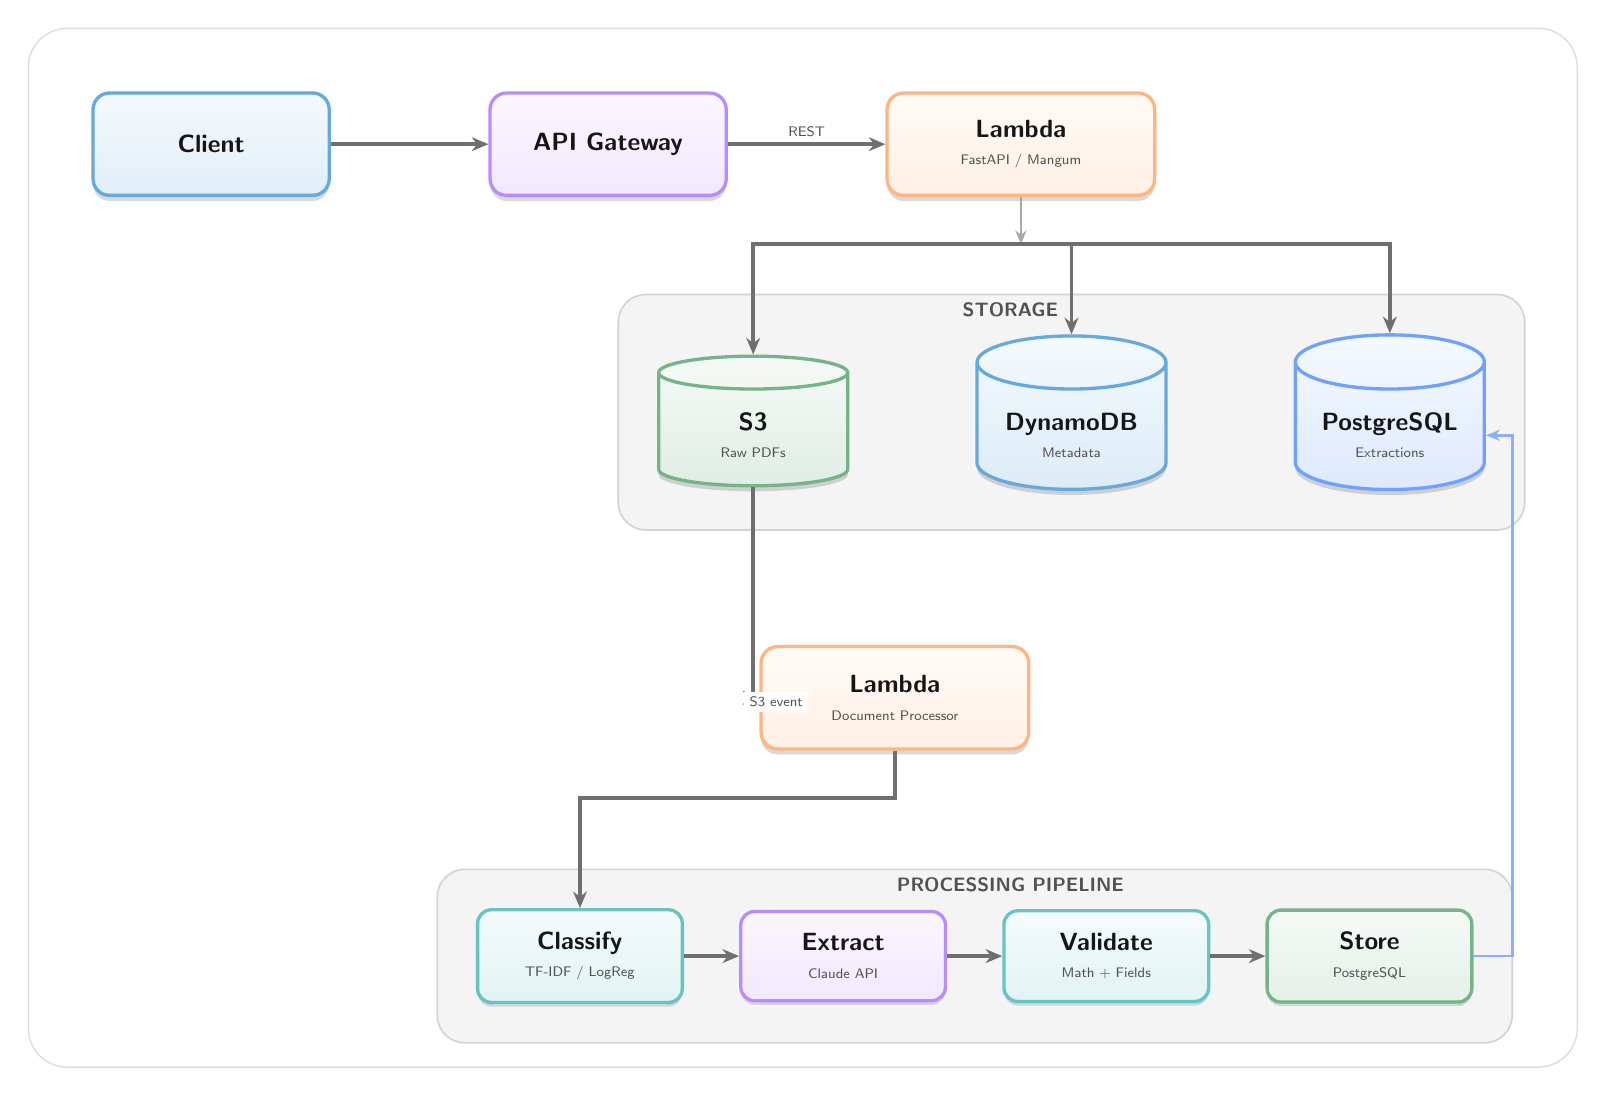
\begin{tikzpicture}

% === ROW 1: Client -> API Gateway -> Lambda ===

\node[service=cyan]
  (client) {\textbf{Client}};

\node[service=purple, right=2cm of client]
  (apigw) {\textbf{API Gateway}};

\node[service=orange, right=2cm of apigw, minimum width=3.4cm]
  (apilambda) {\textbf{Lambda}\\[-1pt]\nsub{FastAPI / Mangum}};

\draw[flow] (client) -- (apigw);
\draw[flow] (apigw) -- node[elabel, above] {REST} (apilambda);

% === ROW 2: Storage ===

\node[stor=green, below=2cm of apilambda, xshift=-3.4cm]
  (s3) {\textbf{S3}\\[-1pt]\nsub{Raw PDFs}};

\node[stor=cyan, right=1.6cm of s3]
  (dynamo) {\textbf{DynamoDB}\\[-1pt]\nsub{Metadata}};

\node[stor=primary, right=1.6cm of dynamo]
  (pg) {\textbf{PostgreSQL}\\[-1pt]\nsub{Extractions}};

% Fan-out arrows from Lambda to storage
\coordinate (fanout) at ($(apilambda.south) + (0,-0.6)$);
\draw[flowlight] (apilambda.south) -- (fanout);
\draw[flow] (fanout) -| (s3.north);
\draw[flow] (fanout) -| (dynamo.north);
\draw[flow] (fanout) -| (pg.north);

% === ROW 3: Processor Lambda ===

\node[service=orange, below=2cm of s3, xshift=1.8cm, minimum width=3.4cm]
  (processor) {\textbf{Lambda}\\[-1pt]\nsub{Document Processor}};

\draw[flow] (s3.south) |- node[elabel, above right, xshift=-4pt, yshift=-6pt] {S3 event} (processor.west);

% === ROW 4: Processing Pipeline ===

\node[step=teal, below=2cm of processor, xshift=-4cm]
  (classify) {\textbf{Classify}\\[-1pt]\nsub{TF-IDF / LogReg}};

\node[step=purple, right=0.7cm of classify]
  (extract) {\textbf{Extract}\\[-1pt]\nsub{Claude API}};

\node[step=teal, right=0.7cm of extract]
  (validate) {\textbf{Validate}\\[-1pt]\nsub{Math + Fields}};

\node[step=green, right=0.7cm of validate]
  (pstore) {\textbf{Store}\\[-1pt]\nsub{PostgreSQL}};

\draw[flow] (processor.south) -- ++(0,-0.6) -| (classify.north);
\draw[flow] (classify) -- (extract);
\draw[flow] (extract) -- (validate);
\draw[flow] (validate) -- (pstore);

% Store -> PostgreSQL feedback
\draw[flowlight, draw=primary!50] (pstore.east) -- ++(0.5,0) |- (pg.east);

% === Background containers ===

\begin{pgfonlayer}{background}
  % Full diagram card background
  \fill[white, rounded corners=14pt]
    ($(current bounding box.south west) + (-0.4,-0.4)$)
    rectangle
    ($(current bounding box.north east) + (0.4,0.4)$);
  \draw[border!40, rounded corners=14pt, line width=0.5pt]
    ($(current bounding box.south west) + (-0.4,-0.4)$)
    rectangle
    ($(current bounding box.north east) + (0.4,0.4)$);

  % Section containers
  \node[container, fit=(s3)(dynamo)(pg),
    label={[clabel]above left:{\textsf{STORAGE}}}
  ] {};

  \node[container, fit=(classify)(extract)(validate)(pstore),
    label={[clabel]above left:{\textsf{PROCESSING PIPELINE}}}
  ] {};
\end{pgfonlayer}

\end{tikzpicture}
\end{document}
